\documentclass[twocolumn]{article}\usepackage[english]{babel}
\usepackage[utf8]{inputenc}
\usepackage{pdfpages}
\usepackage{amsmath}
\usepackage{csquotes}
\usepackage{siunitx}
\usepackage{hyperref}
\usepackage{graphicx}
\usepackage[colorinlistoftodos]{todonotes}
\usepackage[]{mcode}
\usepackage[
backend=biber,
style=alphabetic,
sorting=ynt
]{biblatex}
\addbibresource{bibliography.bib}
\usepackage{tikz}
\usepackage{circuitikz}
\usepackage{placeins}
\title{Using a Lock-In amplifier to determine filters from Low Pass Circuits}
\author{Aaron Kebede}
\date{\today}
\begin{document}
\maketitle
\begin{abstract}

This report provides insight into the analysis of R-C circuits using signal generators. We study circuits in three steps. First, we study a very simple circuit just consisting of a resistor, a capacitor element, and a signal generator. The signal generator generates a current with a specific frequency which we can then vary to study the effects on the other circuit elements. Second, we create a virtual instrument(using LabVIEW) program to automate alteration of the frequency and third, we add a lock-in amplifier in the circuit to extract all the signals and automate our process of collecting the data. We find that for large frequencies, the phase shift is slightly negatively correlated with the frequency while the amplitude has a strong positive correlation. The data, its analysis, and full plots are available at \url{https://220.kebede.org}\footnote{The website contains documentation on how to use the code, how the data is arranged, the nomenclature of the saved data folder}\cite{kebede_2021}

\end{abstract}

\section{Introduction}

Included in this report are details of the method, graphs, results, error analysis, discussions and conclusions of results. We record data and analyze it to find correlations between signals sent from the signal generator and the feedback from the circuit recorded in different sets.  
\newline

\section{Background}
\subsection{RC Circuits}
RC circuits, as the name indicates, are circuits that consist of resistance and capacitance elements. One may think that these circuits would not be of no specific interest, if speaking based solely on how individual resistor and capacitor circuits behave. However, when we have a capacitor and resistor in the same circuit, we start observing some interesting phenomena. One common interesting occurrence is the time constant denoted by the Greek letter, $\tau$(tau). $\tau$ is the product of the capacitance and resistance in the circuit.
\newline
\newline
\newline
\begin{figure}
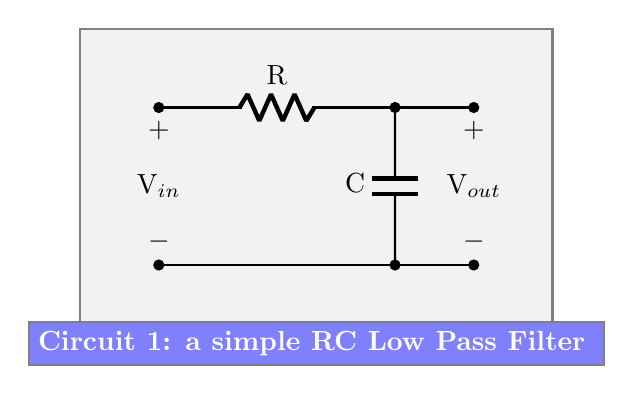
\begin{tikzpicture}[american,thick]
% Change components size
\ctikzset{
    resistors/scale=0.8,
    capacitors/scale=0.7,
}
% Orange boxes
\draw
[
    fill=black!5,
    draw=black!50
] (-1,-0.75) rectangle(5,3);
 
\node
[
    align=center,
    minimum width=6cm,
    fill=blue!50,
    text=white,
    draw=black!50
] at (2,-1){\textbf{Circuit 1: a simple RC Low Pass Filter} };
% Circuit code
\draw (0,0) to[short,*-*] ++ (4,0);
\draw (0,2) to[R=R,*-] ++ (3,0) coordinate(a);
\draw (a) to[short,-*] ++ (1,0);
\draw (a) to[C,l_=C,*-*] ++(0,-2);
% Voltage labels
\draw (0,2) to[open,v=V$_{in}$] ++(0,-2);
\draw (4,2) to[open,v=V$_{out}$] ++(0,-2);
\end{tikzpicture}
\caption{The RC low pass circuit we are studying. In a simple low pass circuit like this one, the voltage first passes through a resistor, only then after,through a capacitor. }
\label{fig:Low Pass Cir}
\end{figure}

The time constant tells us important properties about how the circuit behaves. For instance, we can find out experimentally, how the time constant is related to the voltage drop in the circuit. Although we won't be performing an experiment to verify this(as this is a known fact) in our lab, we can use use some publicly available information to verify this. To do this, we performed a simulation on Circuit Lab\footnote{Circuit Lab is an online Circuit Simulation software}. On Circuit Lab, we created a circuit that emulated the properties and set up of the circuit we had in the lab. We then run the simulation, collected the data and visualized it only to discover that it behaves the same as theoretically predicted.
\newline
\newline
The theoretical prediction of a Voltage charging curve against time is that it will be an exponential curve that relates the voltage at each time with the source voltage. It can be mathematically proven as follows;
Let's apply Kirchhoff's Rule to our circuit in \textbf{Figure 1}.\newline

\(V_{in} - V_{R} - V_{C} =0\), \newline \newline Where V$_{R}$ and V$_{C}$ are voltages in the Resistor and Capacitor respectively. \newline \newline
V$_{C}$ - IR - $\frac{q}{C}$= 0, \newline \newline Where I is the current in the circuit and q is the charge in the capacitor.\newline \newline
V$_{in}$ - R$\frac{dq}{dt}$ - $\frac{q}{C}$ = 0, \newline \newline
$\frac{dq}{dt}$ = $\frac{V_{in}C-q}{RC}$, \newline \newline
\(\int_0^q \frac{dq}{V_{in}C-q} = \frac{1}{RC} \int_0^t dt\), \newline \newline
\text{Simplifying using integration by parts, we get} \newline \newline
\(\frac{V_{in}C - q}{V_{in}C} = e^{-t/RC}\), \newline \newline
\(q(t) = V_{in}C  \left(1 - e^{-\frac{t}{RC}}\right)\) \newline \newline
\(q(t)=Q\left(1 - e^{-\frac{t}{\tau}}\right)\) \newline \newline
\(V(t) = Cq(t)\) \newline \newline
\(V(t)=CQ\left(1 - e^{-\frac{t}{\tau}}\right)\) \newline \newline
\(V(t) = V_{in}\left(1 - e^{-\frac{t}{\tau}}\right)\) ... \textbf{equation 1} \newline \newline
Here, we discover a very important property when V is V($\tau$). This implies that \(V(\tau) = V_{in}\left(1 - \frac{1}{e}\right)\).
\newline \newline
Below are the two voltage curves we made from our simulation - one using a frequency generator and another one as a DC source for the voltage sources. We see in both cases, that the curves follow a general exponential curve. From our derivation above, we have seen that the voltage at any time can be found using equation 1. Our capacitance and resistance values for the circuit were 22nF and \SI{1.5}{M\ohm} respectively from which we can calculate the time constant. \newline
\begin{figure}
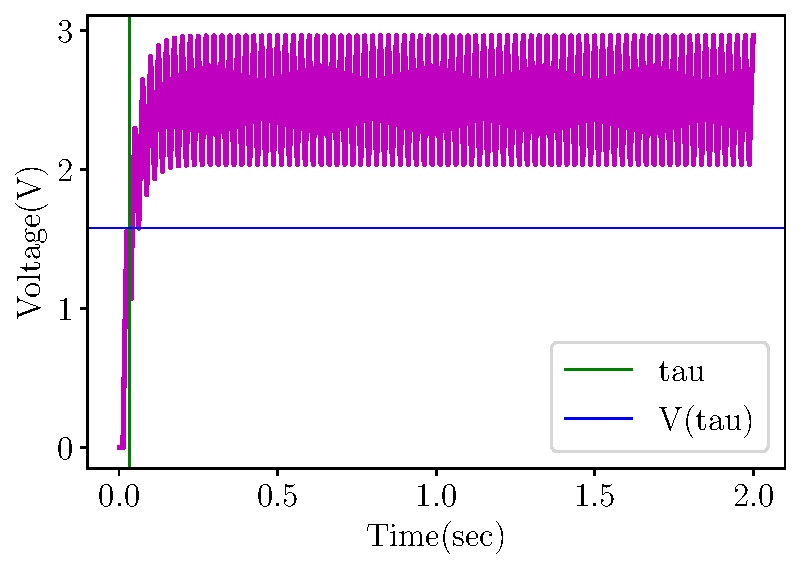
\includegraphics[width=\linewidth]{images/v2/Signal_Generated_RC_Circuit_Plot.pdf}
\caption{\textbf{V} vs \textbf{T} curve in a circuit where the source is signal generated. Although we can see that the signal oscillates between different values at different times, it follows a general exponential path. The theoretical $\tau$ value is indicated with the green vertical line while we indicated the theoretical $V_\tau$ with a blue horizontal line. It can be seen that the two lines indeed actually indeed cross each other at the experimental value of $\tau$}
  \label{fig:Signal RC Voltage}
\end{figure}

\begin{figure}
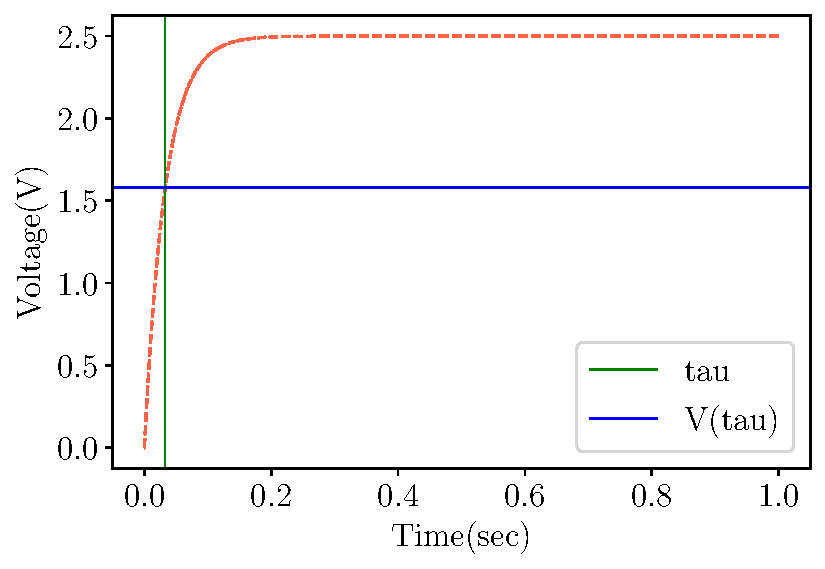
\includegraphics[width=\linewidth]{images/v2/RC_Circuit_Plot.pdf}
\caption{\textbf{V} vs \textbf{T} curve in a circuit where the source is DC voltage. Here, as explained in the \textbf{Figure 2}, we can clearly see that the data matches the very expected values. The labeled \textbf{$\tau$} and \textbf{$V_\tau$} values are theoretical predictions.}
  \label{fig:DC RC Voltage}
\end{figure}

From the curve and experimental data, we can see that the initial voltage
$V_i$ after some time, t, drops to $V_t$. When it is at the time
constant(\textit{i.e.}), t=$\tau$, \newline \newline
\(V(\tau) = V_{in}\left(1 - e^{-\frac{\tau}{\tau}}\right)\) \newline
\(V(\tau) = V_{in}\left(1-\frac{1}{e}\right)\) \newline 

When plotting the experimental data, we labeled the the values of $\tau$ and V($\tau$) to see how the experiment would behave. We find that the experimental results indeed fully match the expected theoretical values as we have presented in Figures 2 and 3. The blue horizontal lines denote V($\tau$) while $\tau$ is represented as the green vertical line on both figures.   
\subsection{Low Pass Circuits}
As the name indicates, a low pass filter is a type of circuit filter that lets low frequency signals pass while impeding high frequency(beyond a certain threshold) signals. Some real life applications of low pass filters include being used as audio filters, or in signal blocking for frequencies above a certain threshold. To construct a low pass filter, we created a circuit that resembles the one that we see at Circuit 1. Theoretically, the way a low pass filter works by leveraging the properties of a capacitor. When designing low pass filters, we connect the signal generator or source first to the resistor. First, since its responses to different input signals are different and secondly, it takes time for a capacitor to charge and discharge as we have seen in the section above. 
When we connect the input directly to the resistor and connect the resistor in series to the resistor, the capacitor lets high frequencies pass while the current below a certain frequency becomes zero. This happens because the capacitor never fully charges at high frequencies but intercepts currents that come out, which blocks current flow in the circuit, but after a certain increase in the frequency, the capacitance decreases and hence current flow is possible.\cite{enwiki:1048317561}
\section{Methods}
\subsection{Set Up and Procedures}
\begin{figure}
  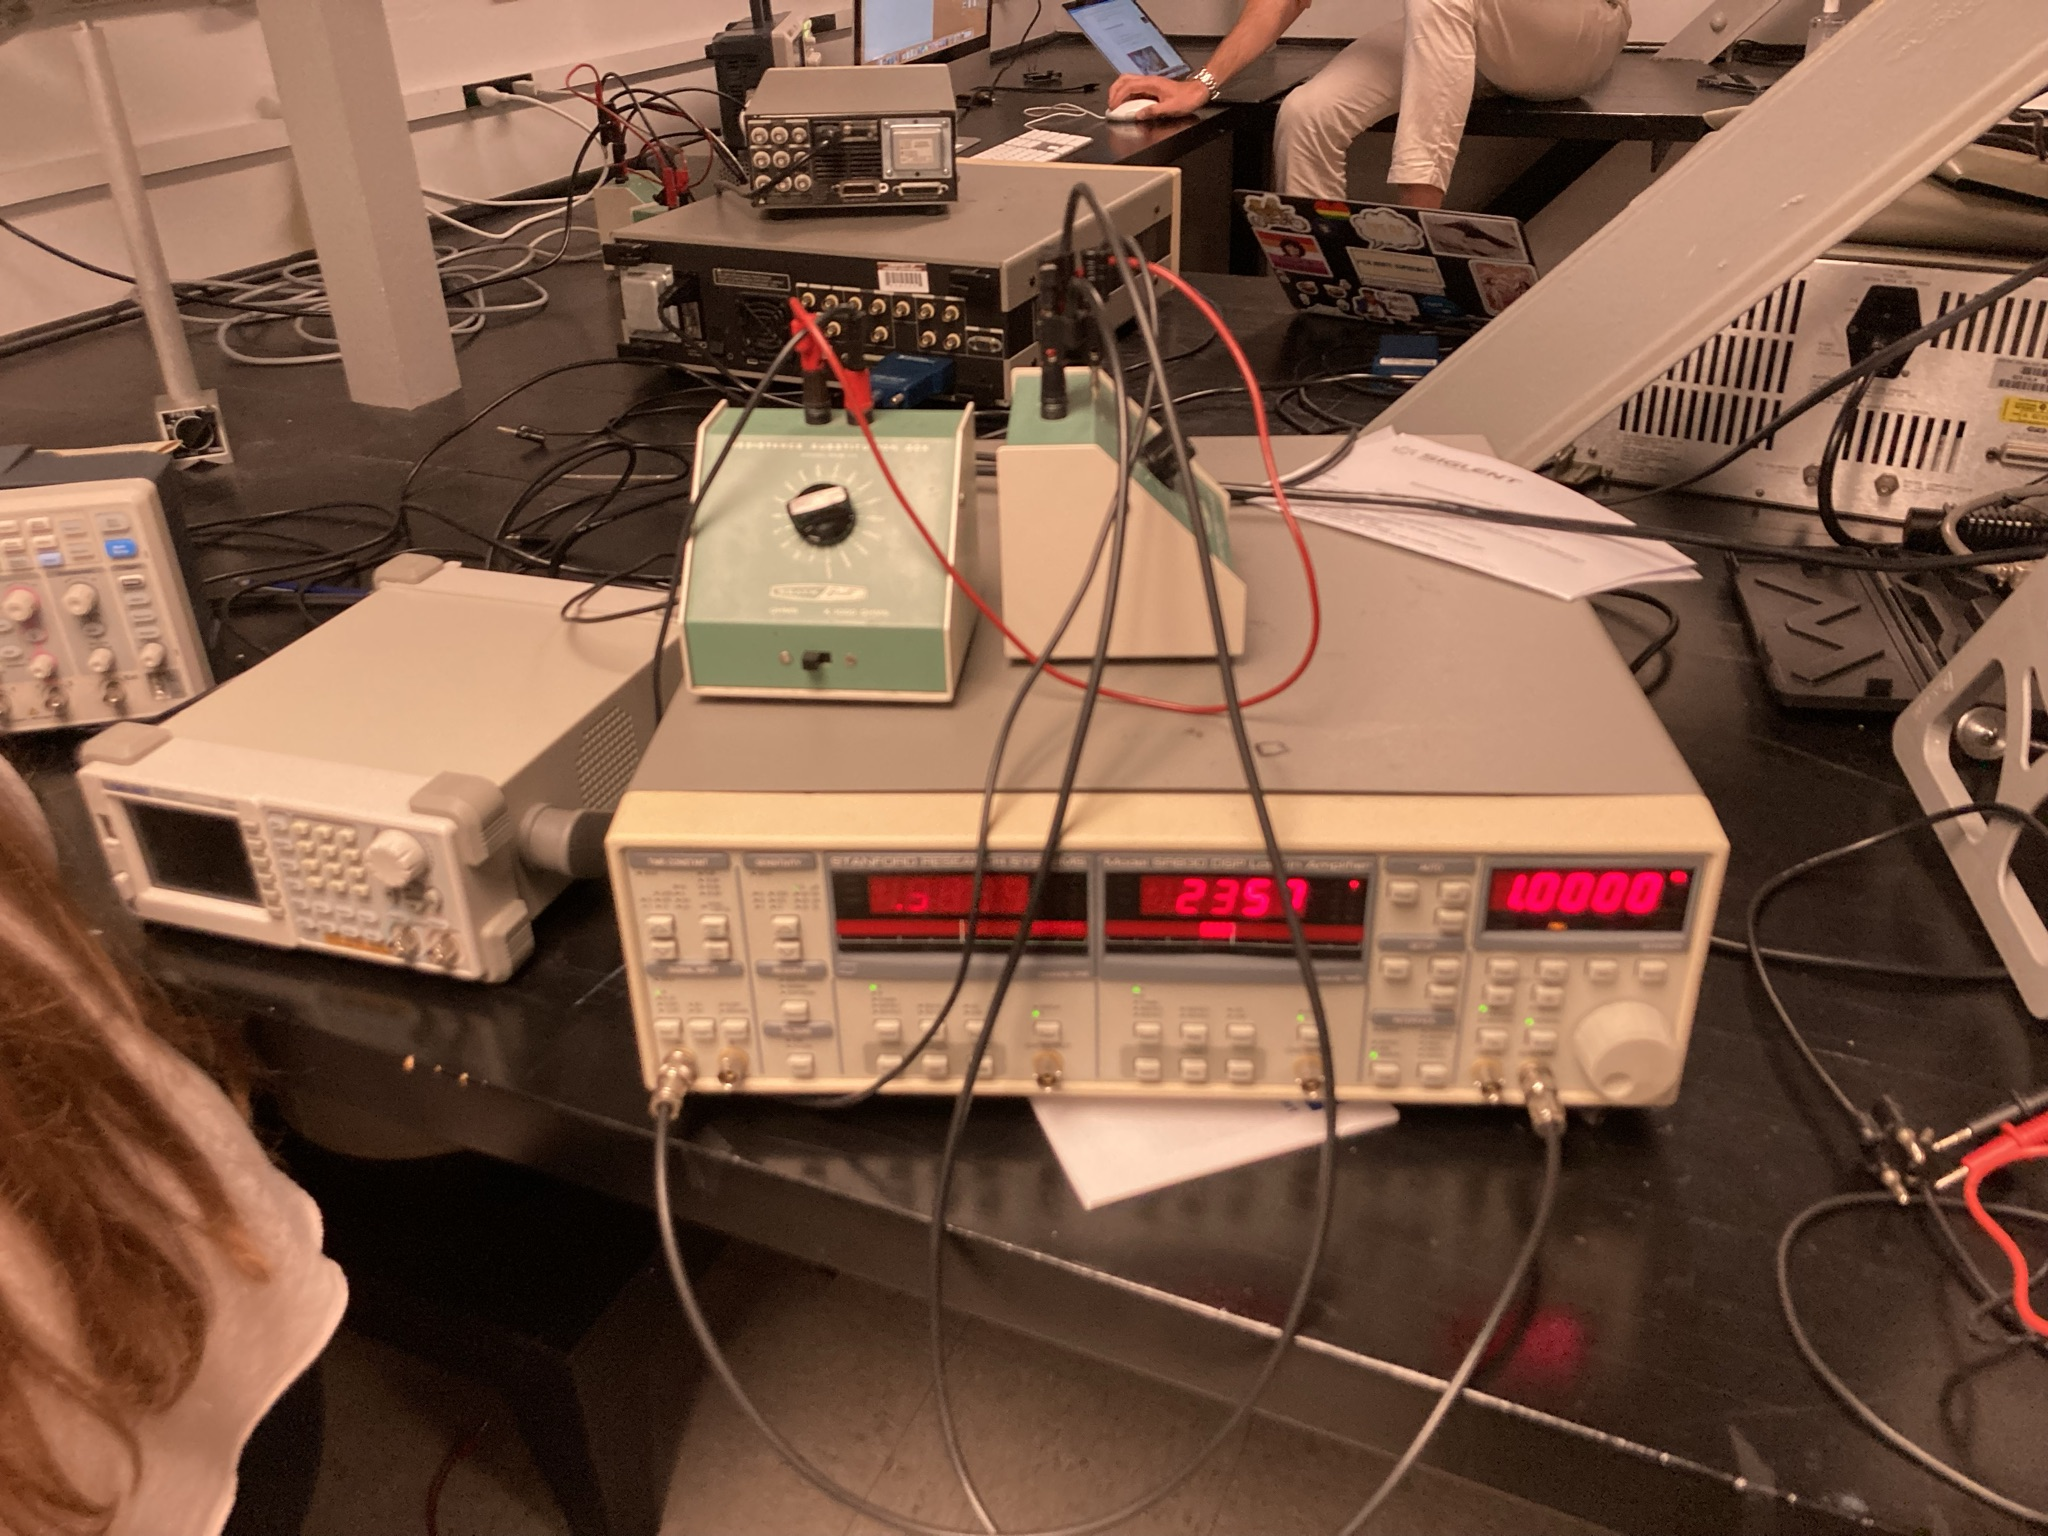
\includegraphics[width=\linewidth]{images/lab/setup.JPEG}
  \caption{Our lab setup}
  \label{fig:LAB_SETUP}
\end{figure}

We performed our data collection in three steps:
\begin{itemize}
\item{\textbf{1.} We set up a circuit with a variable resistor, variable capacitor, and  a function generator. We varied the signal on the function generator and then recorded the data \textbf{by hand} on an excel sheet. Steps like this generally help get started on an experiment and guide on if we are on the right track.} 
\item{\textbf{2.} We then created a LabVIEW program to automate the signals that were being generated. } \item{\textbf{3.} Then, we added an amplifier to the circuit as shown in \textbf{Figure 3} above. We sent signals to the circuit using the LabVIEW program we created in Step 2. We record data automatically into an excel sheet and we start analyzing out output as will be discussed in the \textbf{Results} section.}
\end{itemize}
\subsection{Data Structure}
\begin{tikzpicture}
\node {Root Directory} [sibling distance = 4cm, level distance = 3cm]
    child {node {Hand Recorded Data}} 
    child {node {v1}
    child {node {AMP}}
    child {node {FREQ}}
    child {node {PS}}}
    child {node {v2}
    child {node {LA}
    child {node {P vs F}}
    child {node {A vs F}}}
    child {node {DEF}
    child {node {A vs F}}
    child {node {P vs F}}}};
\end{tikzpicture}
Although we did not use some of the data that was collected, mostly because we were measuring the wrong things or the data sets were too small(as was the case in the hand recorded data), it was a good insight to have on whether we wanted to do the experiment the way it was or if we had to tweak some of the values from the signal generator, or change the capacitance and resistance so that the results we were trying to show would best be represented. As we have explained in the documentation code, organized the data into CSV/XLSX files. Although the default output of the recorded data from LabVIEW is in the excel format, we change the format to CSV in order to make it easier to use it with software libraries like numpy and pandas. We had three major recordings of the data that we categorized into three groups. One is the hand recorded data, the second one is v1, and the third one is v2. v2 is the most recent and main data of the experiment. v1 is the first version of the data that was collected using LabVIEW before incorporating the amplifier in the circuit. We added the amplifier and recollected data into v2. In the latest version, v2, The data is organized into 4 files. Two of the files are \textit{Amplitude vs Frequency} and \textit{Phase Shift vs Frequency}. The other two are the same but with the lock-in amplifier included. \newline \newline \newline \newline \newline \newline \newline \newline \newline \newline \newline \newline \newline \newline \newline \newline \newline \newline \newline \newline \textbf{KEY}
\begin{itemize}

 \item{\textbf{A} / \textbf{AMP} - Amplitude}
 \item{\textbf{F} / \textbf{FREQ} - Frequency }
 \item{\textbf{P} / \textbf{PS}  - Phase Shift}
 \item{\textbf{DEF} - Default(without lock-in amplifier)}
 \item{\textbf{LA} - Lock-in amplifier}
\newline \newline
\end{itemize}
The data output that we will be finally presenting here is calculated using known well known theorems simple formulae. Let's start with the default output (\textbf{DEF}) in the recorded data. The output contains two sets of data, one that measures the Amplitude change due to signal frequency change and another one that measures the Phase Shift due to signal frequency change. Similarly, we created an  identical data structure for the experiment we run with the Lock-In amplifier(\textbf{LA})   

\section{Results and Analysis}

After collecting the data, we performed two  model fits. One using initial guess parameters and another one using a theoretical fit. Each fit was applied for both the Amplitude and Phase Shift curves. We applied model fits and analysis on the latest data set we had(\textbf{v2})
\subsection{Amplitude Curve Analysis}
The first data set that we collected had the amplitude-frequency data. One of the first calculations we performed was to find the cutoff frequency.
The cutoff frequency can be easily found using this relationship:
\(f_{c}=\frac{1}{2\pi\tau}, \) where $\tau$=RC. \newline
In our case,\(\tau=(\SI{1.5}{M\ohm})*(22nF)=0.033\)s, \newline
\(f_c=\frac{1}{2\pi(0.033)}\), which is about 4.82 Hz. This by itself is an indicator of how low our frequency is while we were using signals in the order of tens of thousands. This implies that for frequencies above the cutoff, which is 4.82Hz, the output is significantly low and decreases with increasing frequency.
In figure 5, we have two fits for the observation. The first fit is based solely on the initial values of the parameter. The other fit is based on the the whole data. The latter one fits our observation really well and we can see it very well.
\begin{figure}
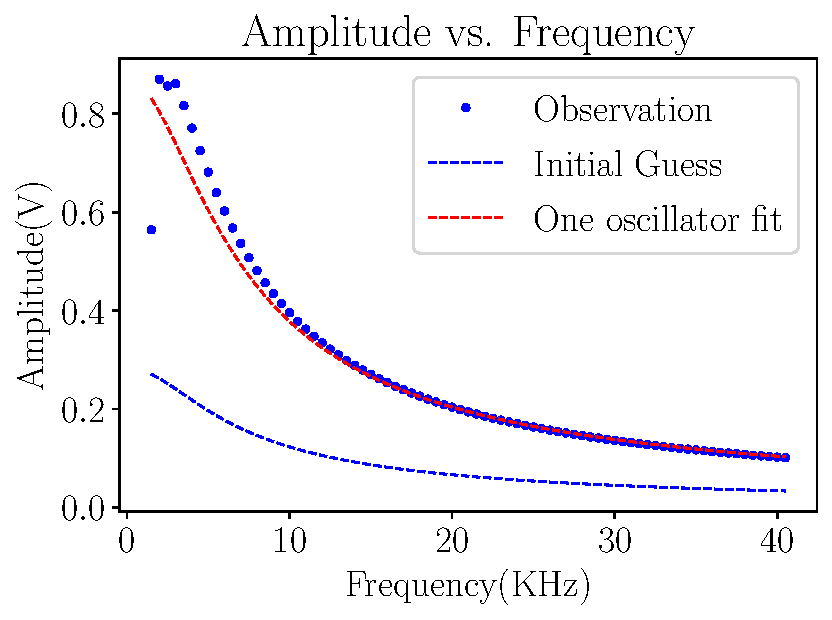
\includegraphics[width=\linewidth]{images/v2/LA_Amplitude_Fit.pdf}
\caption{Lock-in amplifier amplitude fit. In this plot, we have the observation that captures how the amplitude changes with the changing frequency. There is a general trend of decreasing amplitude with increase in the frequency. }
  \label{fig:LA Ampt fit}
\end{figure}
In \textbf{figure 6}, we include the cutoff frequency to visually understand where the frequency stands in the RC filter.

\begin{figure}
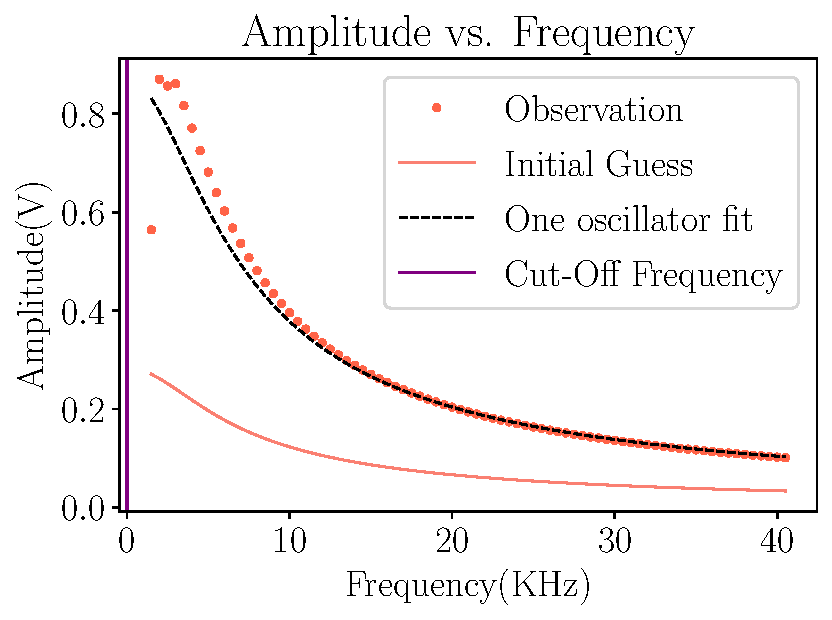
\includegraphics[width=\linewidth]{images/v2/cutoff-fit.pdf}
\caption{Lock-in amplifier amplitude fit with the cutoff frequency labeled. The cutoff frequency at x=0.00482 is labeled with a purple line, and we can see that it is a very small value compared to the range of the frequency(which is 40,000 Hz). The general trend of the amplitude after the cutoff frequency is \textit{decline}, this implies that the voltage is being impeded and hence our filter is rather a low pass one. }
  \label{fig:CutOff LA Ampt fit}
\end{figure}
One important matter to discuss is our fitting functions. For both our amplitude phase(which will be discussed shortly) fits, we used the python package LMFIT\footnote{LMFIT is a python package that express itself as a Non-Linear Least-Squares Minimization and Curve-Fitting for Python}. For the amplitude fit, we used the following fitting formula;
\(fit = \frac{A_m}{\sqrt{(1+(2\pi\tau x)^2}}\), where $A_m$ is the mean amplitude and x is a function we defined as part of the fitting function. You can read more about how the fitting function works on the LMFIT paper\cite{2016ascl.soft06014N}. 
\subsection{Phase Shift Curve Analysis}
As for the phase shift fit, we used the following relation: \newline
\(fit = \frac{P_m}{\pi*arctan(2*\pi*\tau*x)}\), where $P_m$ is the mean phase shift.

When we fit the phase shift to the above function, we get the results shown in figure 7.
\begin{figure}
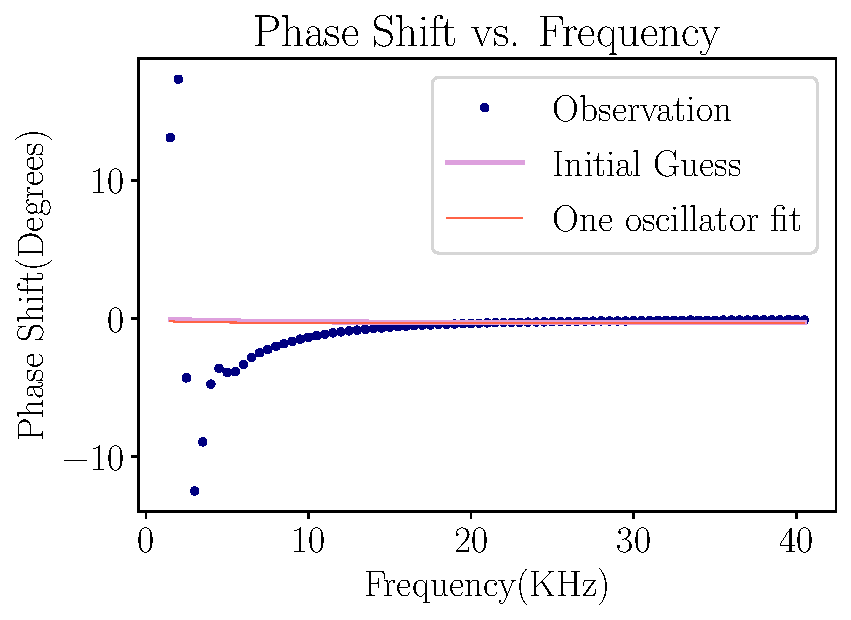
\includegraphics[width=\linewidth]{images/v2/LP_Phase_Shift_Fit.pdf}
\caption{Lock-in amplifier phase shift fit. In this plot, we have the observation that captures how the phase shift changes with the changing frequency. There is a degeneracy between the phase shift and frequency. }
  \label{fig:lp PS  fit}
\end{figure}
As we can observe from figure 8, there is a general degeneracy between the phase shift and the frequency. Although our model worked arguably well in fitting the amplitude, we can see that it doesn't do a great job in fitting for the phase shift. At least, we were expecting a somewhat sinusoidal phase shift as we have seen in the \textbf{DEF} version of the data that we had which is displayed in figure 8.
\begin{figure}
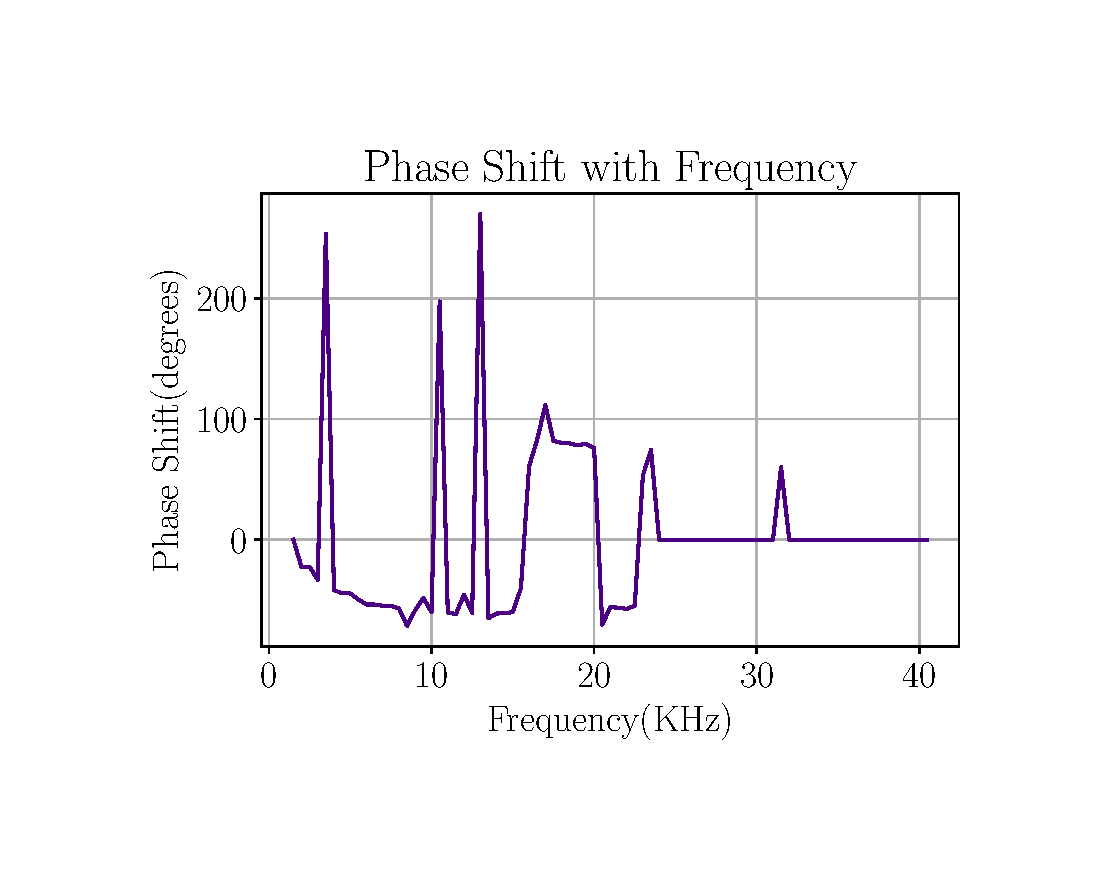
\includegraphics[width=\linewidth]{images/v2/fp.pdf}
\caption{In the \textbf{DEF} version of the data we had, we made a test plot to see   how the phase shift would behave with changing frequency.}
  \label{fig:PS s fit}
\end{figure}
\section{Discussion, Error Analysis and Conclusion}
We observed the theoretically predicted degeneracy between the amplitude and frequency. As for the phase shift fit, there could be many explanations for the not so great phase shift fit that we have. One of the most probable explanations is that we have recorded the wrong thing. We were having difficulties with setting the signal generator and it may have contributed to the possibly faulty data. However, this can't really be a fair explanation to an error. I believe our error stems from the fact that we didn't have enough distinct points for the model to recognize the difference and hence create a fit.

\medskip

\printbibliography
\end{document}